La presente metodología describe el proceso técnico y analítico para la construcción de una plataforma de planificación de trayectorias bajo el paradigma de \enquote{caja blanca}. El enfoque se divide en cinco fases estratégicas que permitirán transitar desde la fundamentación teórica hasta la validación física en hardware comunitario, garantizando la reproducibilidad mediante contenedores y el rigor matemático en variedades toroidales ($T^n$). La Figura \ref{fig:pipeline_metodologia} sintetiza visualmente este flujo de trabajo.

\begin{figure}[htbp]
    \centering
    % !TeX root = ../main.tex
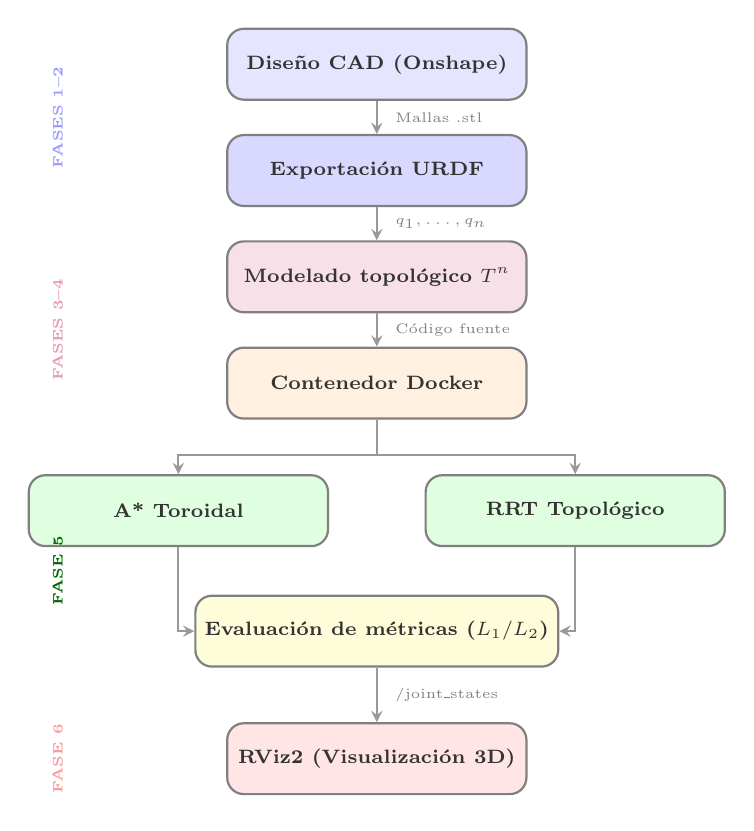
\begin{tikzpicture}[>=stealth, scale=0.9, every node/.style={font=\small},
    % Estilos
    phase/.style={
        draw=black!50, thick, rounded corners=6pt,
        fill=#1, minimum width=3.8cm, minimum height=0.9cm,
        font=\scriptsize\bfseries, align=center, text=black!80
    },
    conn/.style={
        ->, thick, black!40
    },
    lbl/.style={
        font=\tiny, text=black!50
    }
]

% =============================================
% COLUMNA PRINCIPAL (flujo vertical)
% =============================================

% Fase 1
\node[phase=blue!10] (cad) at (0, 0) {Diseño CAD (Onshape)};

% Fase 2
\node[phase=blue!15] (urdf) at (0, -1.5) {Exportación URDF};
\draw[conn] (cad) -- (urdf) node[lbl, midway, right=3pt] {Mallas .stl};

% Fase 3
\node[phase=purple!12] (topo) at (0, -3.0) {Modelado topológico $T^n$};
\draw[conn] (urdf) -- (topo) node[lbl, midway, right=3pt] {$q_1, \dots, q_n$};

% Fase 4
\node[phase=orange!12] (docker) at (0, -4.5) {Contenedor Docker};
\draw[conn] (topo) -- (docker) node[lbl, midway, right=3pt] {Código fuente};

% =============================================
% BIFURCACIÓN: Algoritmos (paralelo)
% =============================================
\node[phase=green!12] (astar) at (-2.8, -6.3) {A* Toroidal};
\node[phase=green!12] (rrt)   at ( 2.8, -6.3) {RRT Topológico};

\draw[conn] (docker.south) -- ++(0,-0.5) -| (astar.north);
\draw[conn] (docker.south) -- ++(0,-0.5) -| (rrt.north);

% =============================================
% CONVERGENCIA: Evaluación
% =============================================
\node[phase=yellow!15] (eval) at (0, -8.0) {Evaluación de métricas ($L_1 / L_2$)};
\draw[conn] (astar.south) |- (eval.west);
\draw[conn] (rrt.south)   |- (eval.east);

% =============================================
% SALIDA FINAL
% =============================================
\node[phase=red!10] (rviz) at (0, -9.8) {RViz2 (Visualización 3D)};

\draw[conn] (eval.south) -- (rviz.north)
    node[lbl, midway, right=3pt] {/joint\_states};

% =============================================
% ETIQUETAS DE FASE (barra lateral izquierda)
% =============================================
\node[rotate=90, font=\tiny\bfseries, blue!40]   at (-4.5, -0.75) {FASES 1--2};
\node[rotate=90, font=\tiny\bfseries, purple!40] at (-4.5, -3.75) {FASES 3--4};
\node[rotate=90, font=\tiny\bfseries, green!40!black]  at (-4.5, -7.15) {FASE 5};
\node[rotate=90, font=\tiny\bfseries, red!40]    at (-4.5, -9.8)  {FASE 6};

\end{tikzpicture}



    \caption{Diagrama de flujo del pipeline metodológico: desde el diseño CAD hasta la validación en hardware físico.}
    \label{fig:pipeline_metodologia}
\end{figure}

\section{Caracterización y construcción del modelo URDF}
El punto de partida de la metodología consistirá en formalizar y ensamblar mecánicamente el \textit{Community Robot Arm}. Se utilizará como base el diseño robótico propuesto por \parencite{community_robot_arm_20sffactory} y los modelos CAD revisados de \parencite{grabcad_robot_arm_2026}. Debido a la limitación de licencias comerciales, el ensamble se migrará íntegramente a \textit{Onshape} \parencite{onshape_cad}, plataforma en la cual se definirán las reglas físicas del modelo (relaciones geométricas \textit{fixed} para bases y uniones \textit{revolute} para los actuadores), estableciendo al mismo tiempo los topes y restricciones de enrutamiento del cableado.

Una vez validado el ensamble cinemático, se exportará al formato \textit{Universal Robot Description Format} (URDF) \parencite{ros_urdf_wiki}. Dicho archivo será sometido a una limpieza estructural, purgando mallas (\textit{meshes}) visuales excesivas, como tornillos, rodamientos y tapas embellecedoras, que sobrecarguen el cómputo de la planificación. La visualización se realizará en RViz2; simular entornos con físicas de gravedad y momento (como Gazebo) recae fuera del alcance de este proyecto.

Para trasladar este modelo articular $(q_1, q_2, \dots, q_n)$ al espacio de trabajo euclidiano, se formulará la cinemática directa (FK) calculando las matrices de transformación de Denavit-Hartenberg \parencite{spong2020robot}, respetando la trazabilidad total del cuerpo robótico en las evaluaciones espaciales.

\section{Modelado matemático del espacio topológico ($T^n$)}
Para construir el entorno de planificación, se trasladará la representación física del manipulador hacia su Espacio de Configuración (\textit{C-Space}). Esta abstracción se dividirá en tres implementaciones lógicas:

\begin{itemize}
    \item \textbf{Construcción de la variedad toroidal:} Puesto que el estado de cada articulación es posicional periódico, cada grado de libertad (GDL) se parametrizará como el grupo topológico circunferencial $S^1$. Al acoplar el mecanismo completo, la dimensión analítica se construirá como el producto cartesiano de estas circunferencias, obteniendo formalmente un Toroide de dimensión $n$:
    \begin{equation}
        T^n = S^1 \times S^1 \times \dots \times S^1 \quad (n \text{ veces})
    \end{equation}
    
    \item \textbf{Implementación de métricas periódicas (\textit{wrap-around}):} Para medir el costo de un movimiento, se codificará un operador de distancia amparado en la topología cociente \parencite{antonyan2016topologia}. Al establecer la relación de equivalencia $\theta \sim (\theta + 2k\pi)$, la función de distancia calculará numéricamente las trayectorias y elegirá la de magnitud mínima, permitiendo saltar la frontera de $360^\circ$ a $0^\circ$.
    
    \item \textbf{Topología del recubrimiento de obstáculos ($\mathcal{C}_{obs}$):} Para evaluar las colisiones, se programará un algoritmo de conversión que transforme objetos intrusivos en subespacios excluyentes mediante aproximación esférica (\textit{Fast Open Approximation of Manifolds}) \parencite{coumar2025foam}. El escenario se modelará mediante aglomeraciones de bolas abiertas, donde la validación topológica $B_r(x) = \{y \in X \mid d(x,y) < r\}$ dictaminará si el manipulador invade una zona prohibida.
\end{itemize}

\section{Arquitectura y virtualización por contenedores}
Buscando erradicar la crisis de reproducibilidad documentada en la robótica y el envejecimiento de las dependencias locales, la arquitectura computacional del proyecto prescinde de instalaciones locales. Toda la plataforma se ensambla dentro de un entorno hermético orquestado, logrando simetrías perfectas de ejecución.
\begin{itemize}
    \item \textbf{Orquestación con Docker Compose:} Se diseña un archivo de despliegue que levanta una imagen base inmutable de Linux (Ubuntu) acoplada con ROS 2 Humble \parencite{macenski2022robot}. Las carpetas del espacio de trabajo (\texttt{ros\_ws}) se montan como volúmenes dinámicos compartidos, permitiendo el desarrollo y compilación ininterrumpidos en tiempo real sin contaminar el sistema operativo del host.
    \item \textbf{Canalización gráfica (X11) y aceleración por GPU:} Para resolver el aislamiento visual tradicional de los contenedores y permitir que el usuario experimente las simulaciones 3D, el orquestador se configura para hacer explícito el puenteo del socket de visualización (\texttt{/tmp/.X11-unix}). Combinado con los perfiles del \textit{NVIDIA Container Toolkit}, el contenedor obtiene autorización matemática para delegar los llamados de renderizado de RViz2 directamente a la GPU local hosteada de las computadoras del laboratorio, manteniendo altas tasas de refresco computacional libre.
\end{itemize}

\section{Implementación de algoritmos \enquote{caja blanca}}
Se descartarán los resolutores comerciales herméticos y se estructurarán analíticamente constructores topológicos medibles: 
\begin{itemize}
    \item \textbf{A* toroidal determinista:} La superficie continua $T^n$ se discretizará en una rejilla celular. El planificador expandirá nodos operando sobre la ecuación $f(n) = g(n) + h(n)$, donde el costo y la heurística se inyectarán con la métrica periódica de $T^n$.
    
    \item \textbf{RRT (\textit{Rapidly-exploring Random Tree}) topológico:} Se desplegará mediante un muestreo aleatorio uniforme en el rango $[0, 2\pi]$. La métrica intervendrá en la búsqueda del vecino más cercano (\textit{Nearest Neighbor}), garantizando que se encuentren atajos matemáticos directos en la configuración.
    
    \item \textbf{Evaluación de colisiones en el continuo:} La validación estructural revisará si el vector arista del movimiento penetra alguna de las bolas abiertas $B_r(x)$ definidas por el modelo FOAM. De suceder una invasión en el subespacio $\mathcal{C}_{obs}$, los planificadores desecharán formalmente la ramificación, garantizando la seguridad en la variedad.
\end{itemize}

\section{Protocolo de evaluación y métricas de desempeño}
Finalmente, para validar rigurosamente la hipótesis de la presente investigación, la propuesta tecnológica completa se someterá a una batería computacional para cuantificar la eficiencia de los planificadores matemáticos aplicados al paradigma de "Caja Blanca". Se medirán explícitamente tres parámetros numéricos y cualitativos:
\begin{itemize}
    \item \textbf{Eficiencia y velocidad computacional (tiempos de CPU):} Se medirá analíticamente el tiempo cronometrado requerido para la convergencia en escenarios sin obstáculos frente a mapas densos. Dicha métrica confirmará el \textit{trade-off} matemático tradicional (un RRT rápido basado en azar, en contraposición al costo elevado del escaneo exhaustivo en el tejido determinista de un A* iterativo).
    \item \textbf{Optimalidad geodésica de la ruta ($L_1$ y $L_2$ acumulados):} Mediante la extracción de las distancias acumuladas en el Espacio de Configuración, se mapeará cuantitativamente la eficiencia por suavidad y economía de movimiento. El A* siempre propondrá recorridos directos exactos (en términos de la métrica Manhattan o Euclidiana seleccionada), por lo que actuará de vara métrica para validar el nivel de oscilación innecesario (\textit{over-shoot}) en las derivaciones probabilísticas de las expansiones RRT en pasillos finos de la variedad.
    \item \textbf{Transferencia física continua y \textit{reality gap}:} Todas las trayectorias de software culminadas serán transferidas y probadas sobre la interfaz del hardware del prototipo comunitario físico ensamblado. El principal evaluador se enfoca en verificar la ausencia de "Jitter" y sobrecargas motrices en los actuadores derivados del efecto "caja mecánica transparente" (vulnerando o conservando la aceleración constante).
\end{itemize}

\section{Cronograma de actividades}
Para dar cumplimiento a los objetivos planteados y responder a 
la pregunta de investigación, se ha diseñado un plan de trabajo 
estructurado en cinco fases estratégicas. Este cronograma abarca un 
periodo de ejecución del 02 de marzo de 2026 al 20 de octubre de 2026, 
contemplando un total estimado de 500 horas de dedicación. El régimen de 
trabajo establecido es de lunes a viernes, en un horario de 16:00 a 19:00 horas, 
lo que permite una dedicación constante y sistemática al desarrollo del proyecto.

La planificación se ha organizado para asegurar una progresión lógica 
desde la fundamentación teórica hasta la validación experimental. En los siguientes 
apartados se describe el desglose detallado de las actividades por fase, mientras 
que la Figura \ref{fig:cronograma_capitular}, ubicada al final de esta sección, ilustra la 
distribución temporal gráfica del proyecto.

\subsection*{Fase 1: Fundamentación y estructuración del proyecto}
El objetivo de esta fase es asentar las bases metodológicas y el rumbo de la investigación, delimitando el problema desde la perspectiva matemática y su impacto en la ingeniería.

\begin{itemize}
    \item \textbf{Redacción del protocolo de investigación} \\
    \textbf{Descripción:} Se redactará el contexto socio-tecnológico, evidenciando la limitación de enseñar robótica mediante simuladores de caja negra. Se justificará la adopción de la robótica topológica como un método analítico superior a la geometría clásica euclidiana. Asimismo, se formularán la pregunta de investigación, la hipótesis basada en el análisis de variedades y los objetivos generales y específicos que guiarán las 500 horas del proyecto.

    \item \textbf{Redacción del cronograma de actividades} \\
    \textbf{Descripción:} Se diseñará la planificación temporal detallada (diagrama de Gantt), distribuyendo estratégicamente la carga de trabajo en bloques de fundamentación, modelado, programación y análisis. Esto garantizará la viabilidad del proyecto y servirá como entregable administrativo para la Carta de Aceptación entre la UnADM y el TESH.
\end{itemize}

\subsection*{Fase 2: Modelado matemático y topológico}
Esta etapa es puramente analítica y teórica. Consiste en la construcción del marco matemático riguroso sobre el cual operará la lógica del software.

\begin{itemize}
    \item \textbf{Revisión del estado del arte} \\
    \textbf{Descripción:} Se realizará un análisis exhaustivo de la literatura científica contemporánea referente a la complejidad topológica en la planificación de trayectorias, contrastando los algoritmos tradicionales de control reactivo frente a los métodos nativos en espacios no contráctiles.

    \item \textbf{Robótica topológica y variedad $T^n$} \\
    \textbf{Descripción:} Se formalizará el espacio de configuración del \textit{Community Robot Arm}. Se demostrará analíticamente que el espacio articular mapea de forma general a un toroide de dimensión $n$ ($T^n$), para posteriormente particularizar su topología métrica intrínseca al caso de tres grados de libertad ($T^3$), eliminando matemáticamente los límites artificiales de los motores (paredes de $0^\circ$ a $360^\circ$).

    \item \textbf{Geometría $\mathcal{C}_{obs}$ y recubrimientos abiertos} \\
    \textbf{Descripción:} Se traducirán los obstáculos físicos del espacio cartesiano a restricciones dentro de la variedad toroidal. En lugar de utilizar cajas delimitadoras (\textit{Bounding Boxes}) computacionalmente costosas, se modelará el subespacio libre de colisiones ($\mathcal{C}_{free}$) mediante el uso analítico de uniones finitas de bolas abiertas, garantizando subespacios topológicamente seguros.

    \item \textbf{Lógica de algoritmos y análisis diferencial} \\
    \textbf{Descripción:} Se evaluará el mapa cinemático directo y se calculará la matriz Jacobiana del manipulador. A través del análisis del determinante, se identificarán las singularidades cinemáticas como inestabilidades topológicas, proveyendo las restricciones lógicas necesarias para que los algoritmos de búsqueda evadan dichos puntos críticos.
\end{itemize}

\subsection*{Fase 3: Desarrollo e implementación de la plataforma}
Fase práctica donde los modelos matemáticos se traducen a código fuente y arquitectura de software.

\begin{itemize}
    \item \textbf{Implementación: Arquitectura de grafos y métricas} \\
    \textbf{Descripción:} Se programarán en Python las estructuras de datos fundamentales para representar el espacio cíclico. Se codificarán las funciones matemáticas de distancia geodésica (\textit{wrap-around}) adaptando las métricas de Manhattan ($L_1$) y Euclidiana ($L_2$) para que operen sin discontinuidades sobre la superficie del toroide.

    \item \textbf{Implementación: Codificación A* ($L_1/L_2$)} \\
    \textbf{Descripción:} Desarrollo desde cero del algoritmo de búsqueda heurística determinista A*. La implementación considerará la discretización del espacio $T^3$ y utilizará las métricas cíclicas previamente definidas para calcular la ruta global más corta, aprovechando la continuidad de la variedad para cruzar fronteras articulares.

    \item \textbf{Implementación: Codificación RRT (Muestreo)} \\
    \textbf{Descripción:} Se codificará el algoritmo de Árboles de Exploración Aleatoria Rápida (RRT). La función de muestreo probabilístico se adaptará para generar nodos sobre la variedad, y la validación de las aristas del grafo se realizará evaluando la pertenencia a los recubrimientos de bolas abiertas, optimizando la detección de colisiones.

    \item \textbf{Desarrollo de paquete de visualización (ROS2/RViz2)} \\
    \textbf{Descripción:} Se desarrollará un paquete personalizado (\textit{custom package}) en ROS2 para la visualización de trayectorias. A diferencia de soluciones estándar como MoveIt, este módulo permitirá proyectar en RViz2 el funcionamiento interno de los algoritmos A* y RRT sobre el modelo tridimensional del \textit{Community Robot Arm}, evidenciando la matemática detrás de la exploración del espacio.
\end{itemize}

\subsection*{Fase 4: Experimentación, validación y análisis}
Periodo de pruebas para extraer datos duros que validen o refuten la hipótesis planteada en la Fase 1.

\begin{itemize}
    \item \textbf{Extracción de datos: Pruebas de conectividad} \\
    \textbf{Descripción:} Se someterá la plataforma a una batería de simulaciones sistemáticas configurando distintos escenarios de obstáculos. Se automatizará la recolección de variables críticas como el tiempo de cómputo, la longitud total de la trayectoria articular y la tasa de convergencia de ambos algoritmos.

    \item \textbf{Análisis de singularidades e inestabilidades} \\
    \textbf{Descripción:} Se mapearán las trayectorias resultantes contra las zonas de singularidad del Jacobiano previamente calculadas. Se verificará matemáticamente que la parametrización de las rutas garantice una evasión natural de los colapsos cinemáticos, demostrando la fiabilidad del modelo.

    \item \textbf{Comparativa estadística de eficiencia (A* vs RRT)} \\
    \textbf{Descripción:} Se realizará un contraste estadístico riguroso entre ambos enfoques. Se evaluará la relación de compromiso (\textit{trade-off}) entre la optimalidad estricta del algoritmo A* en grafos de alta resolución y la superioridad en completitud probabilística y velocidad del RRT en escenarios de alta densidad de obstáculos.

    \item \textbf{Redacción y maquetación de gráficas/resultados} \\
    \textbf{Descripción:} Los datos crudos se procesarán computacionalmente para generar visualizaciones académicas de alta fidelidad, incluyendo representaciones del espacio de configuración toroidal y la visualización de los árboles de búsqueda generados sobre el modelo del robot en RViz2.
\end{itemize}

\subsection*{Fase 5: Consolidación de resultados y cierre}
Etapa final dedicada a la interpretación de los datos y la estructuración del documento.

\begin{itemize}
    \item \textbf{Redacción de hallazgos y comprobación de hipótesis} \\
    \textbf{Descripción:} Se sintetizarán las evidencias empíricas obtenidas para dar respuesta directa a la pregunta de investigación. Se dictaminará si la caracterización topológica y el uso de bolas abiertas lograron una mejora medible en la eficiencia computacional y la seguridad geométrica respecto a los métodos clásicos.

    \item \textbf{Redacción de limitaciones y trabajos futuros} \\
    \textbf{Descripción:} A través de un ejercicio de autocrítica científica, se documentarán los cuellos de botella computacionales del modelo (ej. explosión combinatoria al discretizar). Se propondrán directrices para futuras tesis, como la escalabilidad del algoritmo hacia manipuladores redundantes ($n > 3$ GDL).

    \item \textbf{Revisión final, formato y compilación de Tesis} \\
    \textbf{Descripción:} Se realizará el proceso de edición profunda del documento. Implica la normalización tipográfica en LaTeX, la verificación estricta del formato de citación APA 7 para la bibliografía, la anexión del código base y la generación del PDF final listo para la defensa ante el sínodo evaluador.
\end{itemize}

\begin{landscape}
\begin{figure}[p]
\centering
\vspace*{\fill}
\resizebox{1.3\textwidth}{!}{ % Puedes aumentar el ancho aquí si quieres que ocupe más espacio
\begin{ganttchart}[
    vgrid={*4{black!15, dashed}, *1{black!40, solid}},
    hgrid,
    time slot format=isodate,
    time slot unit=day,
    calendar week text = {\currentweek},
    bar/.append style={fill=blue!40, draw=blue!70},
    bar height=.6,
    group right shift=0,
    group top shift=.7,
    group height=.3,
    group peaks width={0.2},
    x unit=0.17cm,
    y unit title=0.7cm,
    y unit chart=0.8cm,
    title label font=\bfseries\footnotesize,
    bar label font=\footnotesize,
    milestone/.append style={fill=red, draw=red}
]{2026-03-02}{2026-10-20}

\gantttitlecalendar{month, week} \\

% HITO DE INICIO LOGÍSTICO
\ganttmilestone{Firma Carta de Aceptación (CDMX)}{2026-03-05} \\

% FASE 1: INTRODUCCIÓN
\ganttgroup{Fase 1: Fundamentación y estructuración del proyecto}{2026-03-02}{2026-03-08} \\
\ganttbar{Redacción del protocolo de investigación}{2026-03-02}{2026-03-08} \\
\ganttbar{Redacción del cronograma de actividades}{2026-03-02}{2026-03-08} \\

% FASE 2: MARCO TEÓRICO
\ganttgroup{Fase 2: Modelado matemático y topológico}{2026-03-09}{2026-05-15} \\
\ganttbar{Revisión del estado del arte}{2026-03-09}{2026-03-20} \\
\ganttbar{Robótica topológica y variedad $T^n$}{2026-03-23}{2026-04-10} \\
\ganttbar{Geometría $\mathcal{C}_{obs}$ y recubrimientos abiertos}{2026-04-13}{2026-04-24} \\
\ganttbar{Lógica de algoritmos y análisis diferencial}{2026-04-27}{2026-05-15} \\

% FASE 3: METODOLOGÍA
\ganttgroup{Fase 3: Desarrollo e implementación de la plataforma}{2026-05-18}{2026-07-31} \\
\ganttbar{Implementación: Arquitectura de grafos y métricas}{2026-05-18}{2026-06-05} \\
\ganttbar{Implementación: Codificación A* ($L_1/L_2$)}{2026-06-08}{2026-06-26} \\
\ganttbar{Implementación: Codificación RRT (Muestreo)}{2026-06-29}{2026-07-17} \\
\ganttbar{Desarrollo de paquete de visualización (ROS2/RViz2)}{2026-07-20}{2026-07-31} \\

% FASE 4: RESULTADOS Y ANÁLISIS
\ganttgroup{Fase 4: Experimentación, validación y análisis}{2026-08-03}{2026-09-25} \\
\ganttbar{Extracción de datos: Pruebas de conectividad}{2026-08-03}{2026-08-21} \\
\ganttbar{Análisis de singularidades e inestabilidades}{2026-08-24}{2026-09-04} \\
\ganttbar{Comparativa estadística de eficiencia (A* vs RRT)}{2026-09-07}{2026-09-18} \\
\ganttbar{Redacción y maquetación de gráficas/resultados}{2026-09-21}{2026-09-25} \\

% FASE 5: CONCLUSIONES Y CIERRE
\ganttgroup{Fase 5: Consolidación de resultados y cierre}{2026-09-28}{2026-10-20} \\
\ganttbar{Redacción de hallazgos y comprobación de hipótesis}{2026-09-28}{2026-10-06} \\
\ganttbar{Redacción de limitaciones y trabajos futuros}{2026-10-07}{2026-10-13} \\
\ganttbar{Revisión final, formato y compilación de Tesis}{2026-10-14}{2026-10-20}

\end{ganttchart}
}
\captionof{figure}{Cronograma de actividades por fases operativas (Marzo - Octubre 2026).}
\label{fig:cronograma_capitular}
\vspace*{\fill}
\end{figure}
\end{landscape}